
\begin{table*}[t!]

\newcommand{\Tactic}[1]{\multirow{3}{*}{\begin{minipage}{0.1\textwidth}#1\end{minipage}}}
\newcounter{example}
\addtocounter{example}{1}
\newcommand{\id}{\arabic{example} \stepcounter{example}}
\centering
\singlespacing
{\footnotesize
\begin{tabular}{p{0.6ex}|L{0.8\textwidth}|l}
\toprule
& \multicolumn{1}{c|}{Source (S), translation (T) and interpretation (I) text} & Tactic \\
\midrule
\multirow{3}{*}{\id}&\Source{この日本語の待遇表現の特徴ですが英語から日本語へ直訳しただけでは表現できないといった特徴があります.}&\Tactic{\Gn\\\Sg\\\Om}\\
& \Trans{(One of) the characteristics of \moregeneral{honorific} Japanese is that it can not be \moregeneral{adequately} expressed when using a direct translation (from English to Japanese).} & \\
& \Inter{Now let me talk about the characteristic of the Japanese \moregeneral{polite} expressions. $\Segment$ And such such expressions can not be expressed \moregeneral{enough} just by translating directly.} & \\
\midrule
\multirow{3}{*}{\id}&\Source{で三番目の特徴としてはですねえ出来る限り自然な日本語の話言葉とてその出力をするといったような特徴があります.}&\Tactic{\Gn\\\Sm\\\Om}\\
& \Trans{Its third \moregeneral{characteristic} is that its output is, \summarized{as much as possible}, in the natural language of spoken (Japanese).} & \\
& \Inter{And the third \moregeneral{feature} is that the translation could be produced in a \summarized{very} natural spoken language.} & \\
\midrule
\multirow{3}{*}{\id}&\Source{まとめますと我々は派生文法という従来の学校文法とは違う文法を使った日本語解析を行っています.その結果従来よりも単純な解析が可能となっております.}&\Tactic{\Sg\\\Om}\\
& \Trans{In sum , we've conducted an analysis on the Japanese language , using a grammar different from school grammar, called derivational grammar. (As a result,) we were able to produce a simpler analysis (than the conventional method).} & \\
& \Inter{So, we are doing Japanese analysis based on derivational grammar, $\Segment$ which is different from school grammar, $\Segment$ which enables us to analyze in simple way.} & \\
\midrule
\multirow{3}{*}{\id}&\Source{つまり例えばこの表現一は認識できますが二から四は認識できない.}&\Tactic{\Gn\\\Ps\\\Sg}\\
& \Trans{\passivized{They might \moregeneral{recognize}} expression one but not \moregeneral{expressions} two to four.} & \\
& \Inter{The phrase number one only \passivized{is \moregeneral{accepted}} $\Segment$ and \moregeneral{phrases} two, three, four \passivized{were not \moregeneral{accepted}}.} & \\
\midrule
\multirow{3}{*}{\id}&\Source{以上のお話をまとめますと自然な発話というものを扱うことができる音声対話の方法ということを考案しました.}&\Tactic{\Gn\\\Ps\\\Sg}\\
& \Trans{In summary , \passivized{we have \moregeneral{devised}} a way for voice interaction systems \passivized{to handle} natural speech.} & \\
& \Inter{And this is the summary of what I have so far stated. The spontaneous speech \passivized{can be dealt with} by the speech dialog method $\Segment$ and that method \passivized{was \moregeneral{proposed}}.} & \\
\bottomrule
\end{tabular}
}

\caption{Examples of tactics used by interpreters
to cope with divergent word
  orders, limited working memory, and the pressure to produce low-latency translations.  
  We show the source input (S), translated sentences (T), and interpreted sentences (I).
  The tactics are listed in the rightmost column and marked in
  the text:  more general translations are highlighted in
  \moregeneral{italics}; $\Segment$ marks where new clauses or sentences are created;
  and passivized verbs in translation \passivized{are underlined}.
  Information appearing in translation but omitted in interpretation are in (parentheses).
  Summarized expressions and their corresponding expression in translation are \summarized{underlined by wavy lines}.}
  
  
\label{tab:examples}

\vspace{-1em}
\end{table*}
\section{Distinguishing \trans{} and \inter{}}
\label{sec:distinguish}

In this section, we discuss strategies used in \inter{}, which we
detect automatically in the next section.  Our hypothesis is that
tactics used by interpreters roughly fall in two non-exclusive
categories: (i) \emph{delay minimization}, to enable prompt
translation by arranging target words in an order similar to the
source; (ii) \emph{memory footprint minimization}, to avoid
overloading working memory by reducing communicated information.








\paragraph{Segmentation}

Interpreters often break source sentences into multiple smaller
sentences~\cite{erik11theory,shimizu13iwslt}, a process we call segmentation.
This is different from what is commonly used in speech translation
systems~\cite{fujita13timing,oda14segmentation}, where translations of segments
are directly concatenated.  Instead, humans try to incorporate new information
into the precedent partial translation, e.g., using ``which is'' to put it in a
clause (Table~\ref{tab:examples}, Example~3), or creating a new sentence joined
by conjunctions (Table~\ref{tab:examples}, Example~5).

\paragraph{Passivization}

Passivization is useful for interpreting from head-final
languages (e.g., Japanese, German) to head-initial languages (e.g., English,
French)~\cite{he15rewrite}.  Because the verb is needed early in the target sentence but only
appears at the end of the source sentence, an obvious strategy is to wait for the final
verb.  However, if the interpreter uses passive voice, they can start translating
immediately and append the verb at the end (Table~\ref{tab:examples},
Examples~3--4).  During passivization, the subject is often omitted when obvious
from context.


















\paragraph{Generalization}

\newcite{erik11theory} and \newcite{raja00strategy} observe that interpreters
focus on delivering the gist of a sentence rather than duplicating the
nuanced meaning of each word.  More frequent words are chosen as their
retrieval time is faster~\cite{dell92access,cuetos06access} (e.g.,
``honorific'' versus ``polite'' in Table~\ref{tab:examples},
Example~1).  Although \newcite{volansky13feats} show that
generalization happens in translation too, it is likely more frequent
in \inter{} given the severe time constraints.

\paragraph{Summarization}

Faced with overwhelming information, interpreters need efficient ways to
encode meaning.  Less important words, or even a whole sentence can drop,
especially when the interpreter falls behind the speaker.  In
Table~\ref{tab:examples}, Example~2, the literal translation ``as much as
possible'' is reduced to ``very'', and the adjective ``Japanese'' is omitted.

\begin{figure}
\centering
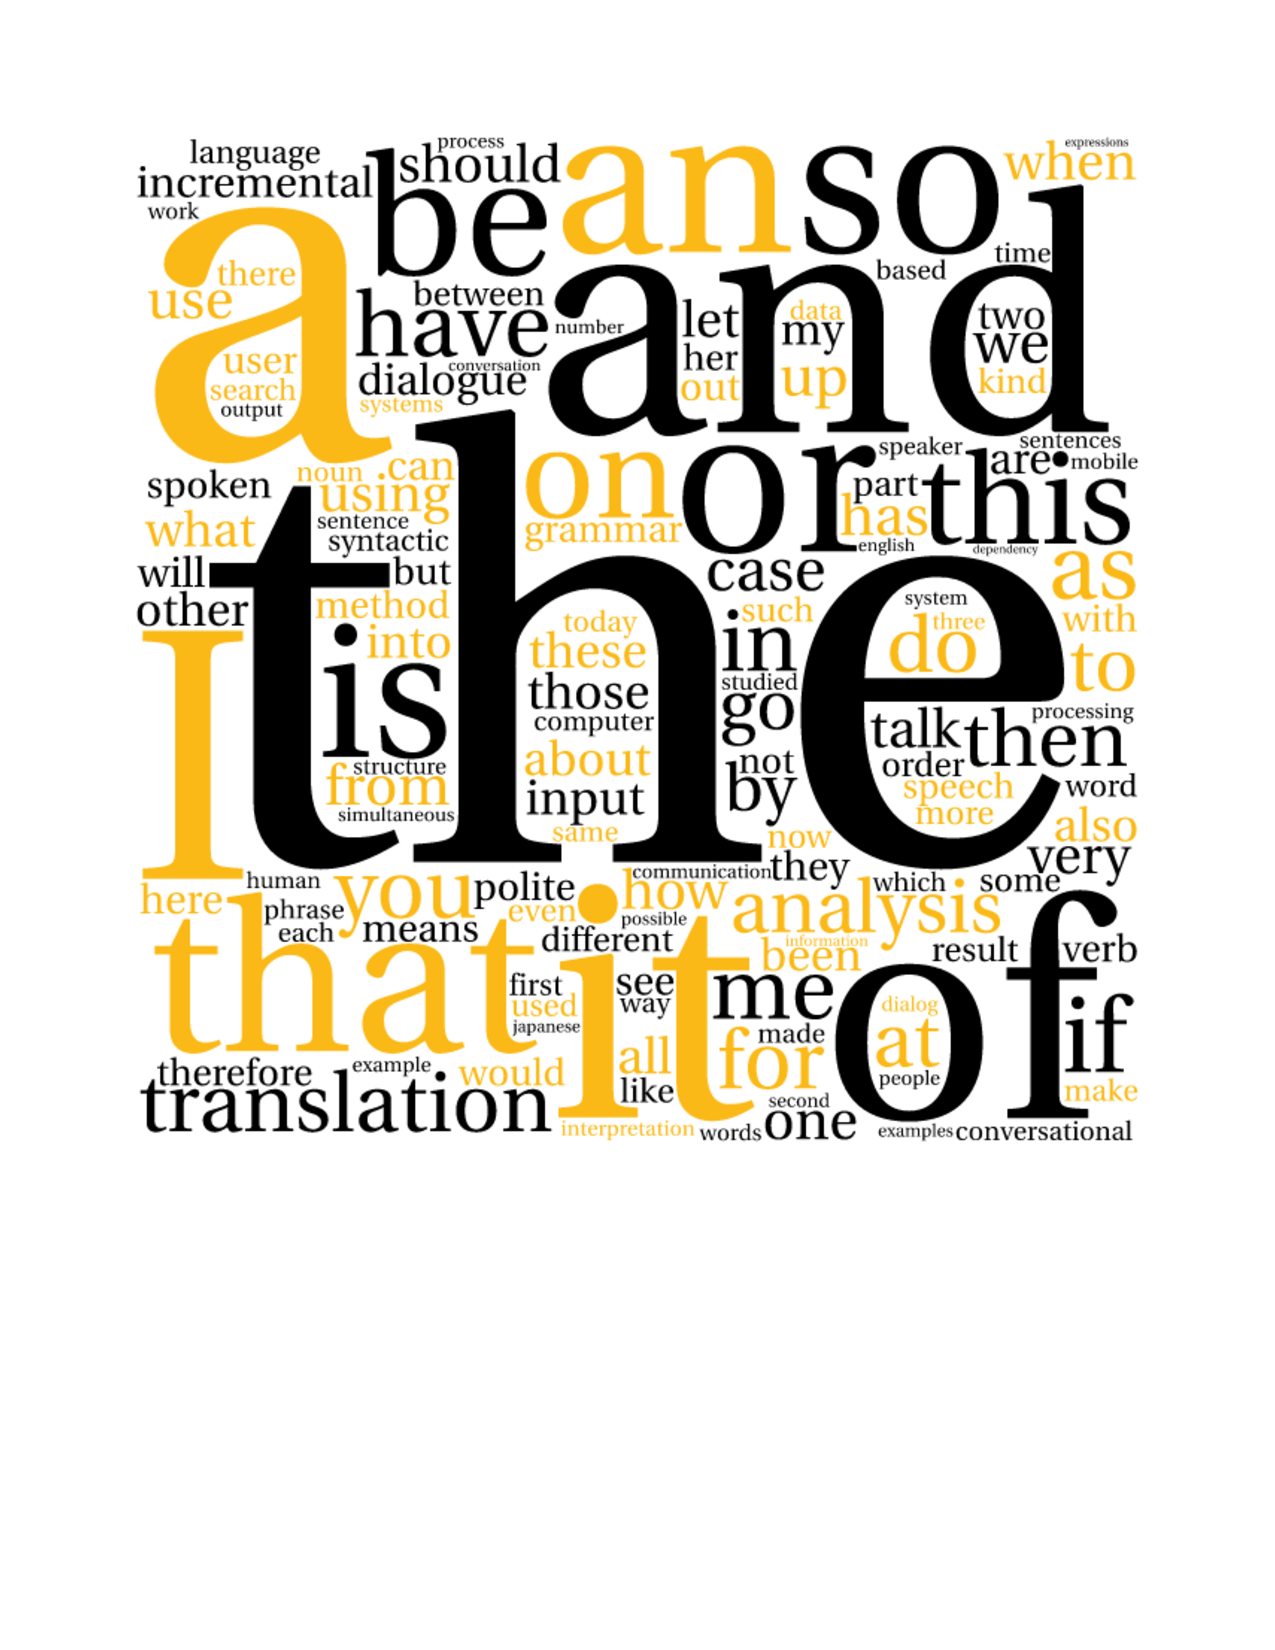
\includegraphics[width=0.7\linewidth]{2016_naacl_interpretese/figures/wordle.pdf}
\caption{A word cloud visualization of \inter{} (black) and \trans{} (gold).}
\label{fig:wordle}
\end{figure}



\paragraph{}

Before we study these characteristics quantitatively in the next section, we
visualize \inter{} and \trans{} by a word cloud in Figure~\ref{fig:wordle}.  The
size of each word is proportional to the difference between its frequencies in
\inter{} and \trans{} (Section~\ref{sec:experiments}).  The word color indicates
whether it is more frequent in \inter{} (blue) or \trans{} (red).  ``the'' is
over-represented in \inter{}, a phenomenon also occurs in \trans{} v.s. the
original text~\cite{eetemadi14feats}.  More conjunction words (e.g., ``and'',
``so'', ``or'', ``then'') are used in \inter{}, likely for segmentation, whereas
``that'' is more frequent in \trans{}---a sign of clauses.  In addition, the
pronoun ``I'' occurs more often in \trans{} while ``be'' and ``is'' occur more
often in \inter{}, which is consistent with our passivization hypothesis.
